\section{Evaluation}\label{sec:eval}

We ask five questions. Does FOA follow honest drift (liveness)? Does it stop poisoning, in particular
poisoning hidden inside drift (safety)? Does vulnerability diversity matter against a monoculture
botnet? Is it immune to the freeze attack and to attacks on its gossip? And what does it cost?

\subsection{Setup}\label{sec:setup}

\textbf{Traffic.} We use all nine devices of N-BaIoT~\cite{nbaiot}: two doorbells (Danmini, Ennio), a
thermostat (Ecobee), a baby monitor (Philips), four security cameras (Provision PT-737E and PT-838,
SimpleHome XCS7-1002 and -1003) and a webcam (Samsung), each with its real benign capture and its real
Mirai and BASHLITE attack traffic (Ennio and Samsung have BASHLITE only). Each row is the 115 Kitsune
statistics of one packet~\cite{kitsune}. The first 20\% of each benign capture calibrates the device's
detector; the rest streams in capture order, alternate rows for learning and for measuring false alarms.
Each attack type is split into a pool the poisoner draws from and a disjoint held-out set on which
detection is measured. The shared 16-dimensional whitened basis keeps \ExplainedVar\ of the within-device variance.

\textbf{Fleet.} The main fleet has the nine devices, one each; peers are all devices of other vendors.
For the monoculture experiment a twelve-device fleet has three instances each of four models; instances
differ in calibration subsample, position in the capture and random seed.

\textbf{Honest drift.} We apply drift to the raw Kitsune statistics with physical meaning: packet rate
$\times g$ (counts scale by $g$, inter-packet gaps by $1/g$), $b$ bytes of per-packet overhead in both
directions (a tunnel or a new record layer), and network jitter $\times h$. Attack traffic gets the
overhead and jitter (same network path) but not the benign rate change. Kitsune's log-scaled
statistics barely move under small changes (packet rate $\times 8$ raises a static detector's false
alarms only to 22\%), so drift strength was fixed by its effect on the static detector alone, never by
how any adaptive rule behaves. \emph{Strong} common drift ($g=64$, $b=240$, $h=11.4$, ramped over cycles 40
to 160) takes the static detector to \StrongStaticFPR\ false alarms; \emph{moderate} ($g=16$, $b=160$,
$h=5$) to about a third. Device-only drift ($g=32$, $b=200$, $h=7.6$, cycles 60 to 120) models one
device's own large change. These are stress tests of a large shared change; Section~\ref{sec:cesnet}
uses real drift.

\textbf{Attacker.} The poisoner targets the victim's scan traffic (Mirai scan, or BASHLITE scan on the
two devices without Mirai), the attack class closest to benign traffic, from cycle 40 on, with share
$p\in\{0.1,0.2,0.3,0.4\}$ of the victim's learning batch. Modes: \emph{boundary} (real benign points
pulled toward real attack points until just inside the alarm radius), \emph{core} (just inside the core
radius), \emph{mimicry} (re-centred copies of benign traffic shifted toward the attack, which looks like
drift to the device), \emph{multi-direction}, \emph{consensus-aligned} and \emph{pulsing}.

\textbf{Baselines.} All rules share the same detector and the same local proposal, so differences come
from how the proposal is applied. \emph{Static} never adapts. \emph{Naive} applies a mean-and-radius
proposal over all accepted traffic. \emph{Single-device} applies our signature-free proposal in full.
\emph{Clipping} caps each update's norm (robust-aggregation-style clipping with no memory).
\emph{Frozen reserve} learns only from points a frozen copy of the calibrated detector accepts
(WARDEN-style screening~\cite{warden}). \emph{Alarm-rate switch-off} skips updates while the batch alarm
rate exceeds five times the clean rate (Kloft and Laskov~\cite{kloft}). \emph{Outlier-ratio gate} skips
updates while the alarm rate exceeds three times its own moving average (DriftXpert style~\cite{driftxpert}).
\emph{TOA} is our earlier rule that rations movement toward an \emph{oracle} attack signature.
\emph{Same-model consensus} applies the element-wise median of same-model devices' proposals and discards
the rest (CIoTA style~\cite{ciota}). The gates are our re-implementations of the gating idea in each
paper, not the full published systems.

\textbf{Metrics.} A victim is \emph{compromised} when fewer than half of held-out target attack packets
are flagged; time to compromise (TTC) is the first such cycle. False-alarm rate (FPR) is measured on
held-out benign traffic each cycle, on the victim and on the rest of the fleet. All results are over 10
seeds (95\% confidence intervals where shown); a run is 240 cycles of 200 learning points per device.


\textbf{Protocol hygiene.} Design choices (the robust agreement, the spread budget, the drift strength
and the victim rule) were made on development seeds 0 and 1; every number below uses held-out seeds
2 to 11. A device is a victim only if its target attack sits at least 1.3 alarm radii from its own
benign traffic under the calibrated static detector (median score over $\tau$). Philips (1.04) and
SimpleHome XCS7-1002 (1.16) fail this test; no centroid detector protects an attack that close for
long, and they remain in the fleet as peers. Finally, honest drift by itself can carry benign traffic
into an attack region: on one camera, even an attacker-free run loses its scan detection under strong
drift. Every attacked run is therefore paired with the same run without the attacker, and a victim
counts as compromised only when it loses detection that its attacker-free twin keeps.

\subsection{Liveness: following honest drift}
Table~\ref{tab:liveness} and Figure~\ref{fig:liveness} show false alarms with no attacker. Under strong
shared drift a static detector reaches \StrongStaticFPR. Every gate that pauses learning on a suspicious
statistic pays for it: the alarm-rate switch-off and the frozen reserve end at \GateFleetFPR. FOA ends at
\FOAFleetFPR, below even single-device adaptation (\AutoFleetFPR), because the fleet consensus is a less
noisy estimate of the shared drift than any one device's batch. Only naive learning, which accepts
everything and is trivially poisoned, is lower (\NaiveFleetFPR). The price shows under device-only
drift: FOA admits a device's own change only at rate $B$, so that device ends at \FOAIdioFPR\ false alarms
against \AutoIdioFPR\ for single-device adaptation. This is Proposition~\ref{prop:frontier} made
visible, and Section~\ref{sec:frontier} shows how $B$ moves it.

\begin{figure*}[t]
\centering
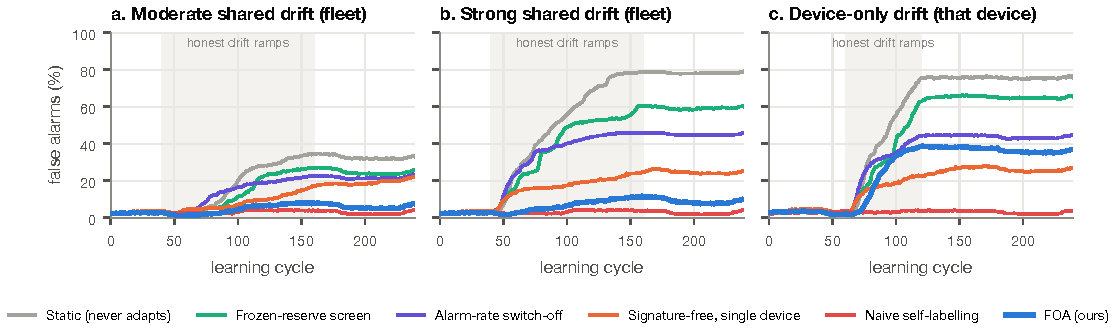
\includegraphics[width=\textwidth]{figures/fig_liveness.pdf}
\caption{False alarms with no attacker (10 held-out seeds). Shared drift (a, b) is followed by FOA through
the consensus; device-only drift (c) is admitted only at the residual rate $B$, the cost predicted by
Proposition~\ref{prop:frontier}.}
\label{fig:liveness}
\end{figure*}

\subsection{Safety: poisoning hidden inside drift}
With no drift (Table~\ref{tab:e2}), the signature-free local rule already resists most attackers
(\NoDriftAutoComp\ compromised against \NoDriftNaiveComp\ for naive learning), and FOA keeps that
(\NoDriftFOAComp). Drift is what breaks single-device defences: during a strong shared drift the
detector must move, and a poisoner moves with it. Table~\ref{tab:e3} and Figure~\ref{fig:headline}
show the result over \NRunsEThree\ runs. Against the classic boundary attacker FOA is compromised in
\FOABoundaryComp\ of runs at every share, against \AutoBoundaryComp\ for single-device adaptation (up to
\AutoBoundaryCompHigh\ at share 0.4). Over all three attacker types FOA is compromised in \FOAComp\ of
runs, single-device adaptation in \AutoComp, the alarm-rate switch-off in \KLComp\ and the frozen reserve
in \FrozenComp. Only TOA does better (\TOAComp), because it is handed the true attack signature, and it
pays for it with false alarms. FOA is the only rule in the lower-left corner of
Figure~\ref{fig:headline}b: few compromises \emph{and} few false alarms.

FOA is not unbreakable. A core-hiding attacker at share 0.4 compromises \FOACoreHigh\ of victims and a
mimicry attacker \FOAMimicHigh, almost all on the two Provision cameras, whose scan traffic is the
closest to benign among our victims. When FOA is compromised it takes longer: a median of \FOAMedTTC\
cycles after poisoning starts, against \AutoMedTTC\ for single-device adaptation. The bound of
Corollary~\ref{cor:ttc} was checked in every cycle of every attacked FOA run here and was violated
\BoundViolations\ times.

\begin{figure*}[t]
\centering
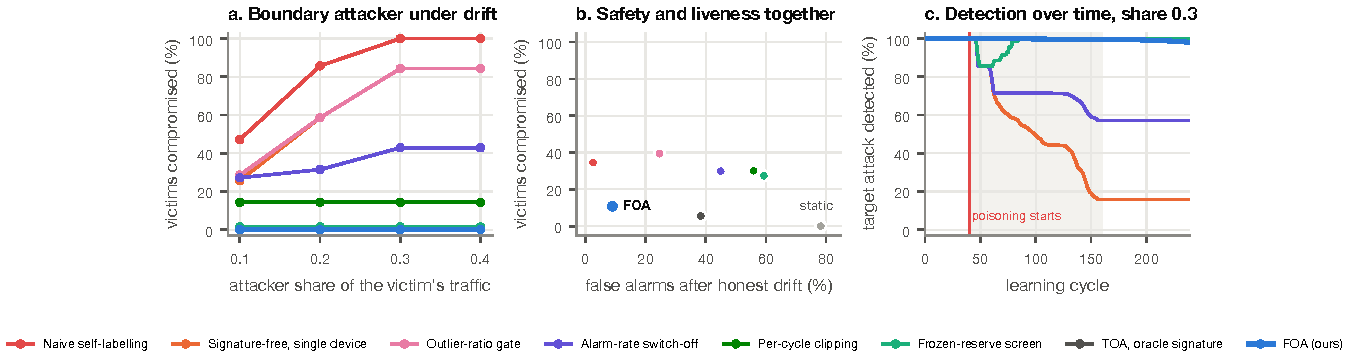
\includegraphics[width=\textwidth]{figures/fig_headline.pdf}
\caption{Poisoning hidden inside strong shared drift (7 victims, 10 held-out seeds, compromise counted
against an attacker-free twin). (a) Boundary attacker: FOA is never compromised. The outlier-ratio gate
never fires here and coincides with single-device adaptation. (b) Overall compromise against false
alarms after drift: FOA alone is low on both. (c) Mean detection of the target attack over time.}
\label{fig:headline}
\end{figure*}

% Generated by make_numbers.py. Do not edit.
\begin{table}[t]
\centering
\caption{False alarms (\%) after honest drift, no attacker. Shared drift: fleet mean; device-only: that device. 10 held-out seeds.}
\label{tab:liveness}
\small
\setlength{\tabcolsep}{4pt}
\begin{tabular}{@{}lrrr@{}}
\toprule
Rule & Moderate & Strong & Device-only \\
\midrule
Static & 32.7 & 78.3 & 75.6 \\
Naive & 2.6 & 2.6 & 2.6 \\
Single device & 18.9 & 24.6 & 26.0 \\
Clipping & 22.3 & 55.9 & 61.3 \\
Frozen reserve & 24.7 & 59.3 & 65.0 \\
Alarm switch-off & 21.7 & 45.0 & 43.5 \\
Outlier-ratio gate & 18.3 & 24.6 & 26.7 \\
TOA (oracle) & 28.5 & 38.3 & n/a \\
\textbf{FOA} & 6.0 & 9.0 & 36.1 \\
\bottomrule
\end{tabular}
\end{table}

\begin{table}[t]
\centering
\caption{Attack hidden in strong shared drift: victims compromised (\%, attack-attributable) by attacker type, averaged over shares 0.1 to 0.4, and false alarms after drift (\%). 7 victims, 10 held-out seeds.}
\label{tab:e3}
\small
\setlength{\tabcolsep}{4pt}
\begin{tabular}{@{}lrrrrrr@{}}
\toprule
Rule & Bound. & Core & Mimic. & All & FPR$_v$ & FPR$_{fl}$ \\
\midrule
Naive & 83 & 18 & 2 & 35 & 1.1 & 2.6 \\
Single device & 63 & 37 & 18 & 39 & 10.3 & 23.8 \\
Outlier-ratio gate & 64 & 37 & 18 & 39 & 10.5 & 23.8 \\
Alarm switch-off & 36 & 36 & 18 & 30 & 42.2 & 43.4 \\
Clipping & 14 & 46 & 30 & 30 & 51.0 & 54.0 \\
Frozen reserve & 1 & 52 & 28 & 27 & 66.6 & 57.2 \\
TOA (oracle) & 0 & 10 & 6 & 5 & 41.1 & 37.0 \\
\textbf{FOA} & 0 & 15 & 18 & 11 & 10.2 & 7.3 \\
\bottomrule
\end{tabular}
\end{table}

\begin{table}[t]
\centering
\caption{Poisoning with no drift: victims compromised (\%) by attacker type, averaged over shares 0.1 to 0.4.}
\label{tab:e2}
\small
\setlength{\tabcolsep}{4pt}
\begin{tabular}{@{}lrrrr@{}}
\toprule
Rule & Boundary & Core & Mimicry & All \\
\midrule
Naive & 86 & 21 & 1 & 36 \\
Single device & 0 & 15 & 7 & 7 \\
Alarm switch-off & 0 & 15 & 7 & 7 \\
Clipping & 0 & 14 & 1 & 5 \\
Frozen reserve & 0 & 9 & 3 & 4 \\
TOA (oracle) & 0 & 4 & 0 & 1 \\
\textbf{FOA} & 0 & 7 & 7 & 5 \\
\bottomrule
\end{tabular}
\end{table}

\begin{table}[t]
\centering
\caption{One knob: residual slope $B$ (alarm radii per cycle). Victims compromised under strong drift (boundary attacker, share 0.4, 4 victims) and false alarms after device-only drift (\%).}
\label{tab:sweep}
\small
\setlength{\tabcolsep}{4pt}
\begin{tabular}{@{}lrr@{}}
\toprule
$B$ & Compromised & Device-only FPR \\
\midrule
0.00125 & 0 & 55 \\
0.0025 & 0 & 43 \\
0.005 & 0 & 31 \\
0.01 & 50 & 29 \\
0.02 & 50 & 11 \\
0.04 & 75 & 16 \\
Single device & 75 & 20 \\
Alarm switch-off & n/a & 21 \\
Frozen reserve & n/a & 55 \\
Static & n/a & 65 \\
\bottomrule
\end{tabular}
\end{table}

\begin{table}[t]
\centering
\caption{Ablations under strong shared drift (3 victims, 10 seeds): victims compromised by a boundary attacker at share 0.3 (\%), fleet false alarms after drift (\%), and false alarms on a device with its own drift on top of the shared one (\%).}
\label{tab:ablation}
\small
\setlength{\tabcolsep}{4pt}
\begin{tabular}{@{}lrrr@{}}
\toprule
Variant & Comp. & FPR$_{fl}$ & FPR$_{own}$ \\
\midrule
FOA (default) & 0 & 7.0 & 90 \\
mean instead of geometric median & 0 & 5.9 & 74 \\
coordinate-wise median & 0 & 6.9 & 90 \\
mean-based agreement & 0 & 13.8 & 90 \\
no agreement ($\lambda=1$) & 0 & 11.5 & 90 \\
no significance ($w=1$) & 0 & 10.1 & 90 \\
no common budget & 0 & 7.0 & 90 \\
2$\times$ wider spread budget & 33 & 10.0 & 90 \\
joint centre+spread budget & 33 & 15.2 & 42 \\
no residual budget & 67 & 23.4 & 57 \\
discard residual (CIoTA-like) & 0 & 53.6 & 100 \\
no peers (budget only) & 0 & 43.0 & 100 \\
2 diverse peers & 7 & 9.7 & 80 \\
3 diverse peers & 3 & 8.6 & 80 \\
3 random peers & 3 & 8.1 & 81 \\
all peers & 0 & 7.2 & 90 \\
\bottomrule
\end{tabular}
\end{table}



\subsection{Monoculture botnets: why the peers must be diverse}
The twelve-device fleet has three instances each of four models. A botnet infects $k$ of the three
SimpleHome XCS7-1003 cameras and poisons all of them together during strong drift
(Figure~\ref{fig:monoculture}; without drift no rule was compromised). Same-model consensus, as in CIoTA~\cite{ciota}, works while the
infected cameras are a minority of their group: with one of three infected it is compromised in
\MonoCiotaOne\ of runs. Once two or three of the three are infected, the consensus \emph{is} the botnet,
and it is compromised in \MonoCiotaThree\ of runs; FOA restricted to same-model peers fails the same way
(\MonoSameThree). FOA with vulnerability-diverse peers is compromised in \MonoFOAThree\ of runs at every
$k$, as is FOA listening to all peers, because one exploit reaches at most three of eleven peers. This
is the head-to-head that separates FOA from same-model consensus. In this fleet, diversity has a cost:
a device whose only diverse peers are three other models gets a coarser consensus and higher false
alarms than one listening to all peers, so in practice a peer group should be as large as possible
subject to no single vulnerability class holding half of it.

\begin{figure}[t]
\centering
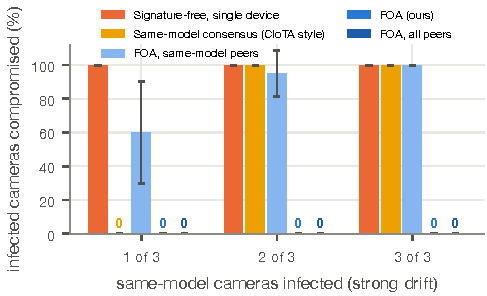
\includegraphics[width=\columnwidth]{figures/fig_monoculture.pdf}
\caption{Monoculture botnet: $k$ of three same-model cameras are infected and poisoned together.
Same-model consensus fails as soon as the infected cameras are a majority of their model; FOA with
diverse peers does not.}
\label{fig:monoculture}
\end{figure}

\subsection{The freeze attack}
An attacker sends loud decoy traffic (real attack packets, pushed out to twice the alarm radius) to one
device from cycle 40 to 100, while strong honest drift runs from cycle 40 to 160, and then leaves
(Figure~\ref{fig:freeze}). Decoys are never learned from by any rule; their only possible effect is on a
stop-learning gate. The alarm-rate switch-off closes as soon as decoys arrive, honest drift moves on
without it, and when the attacker leaves the alarm rate stays high because the traffic has drifted
away: the gate never reopens and the device ends at \KLFrozenFPR\ false alarms, against \KLCleanFPR\
for the same gate without the attacker, at every decoy share from 5\% upward. Not every gate freezes:
the outlier-ratio gate compares the alarm rate with its own moving average, which rises with the decoys,
so it reopened and ended where it would have without the attacker (\ORFrozenFPR); the frozen reserve has
no gate to trip but suffers from the drift itself. FOA's trajectory is unchanged (\FOAFreezeFPR\ with the attacker,
\FOAFreezeClean\ without), exactly as Proposition~\ref{prop:freeze} states; our unit tests check that the
two trajectories are bit-for-bit identical.

\begin{figure*}[t]
\centering
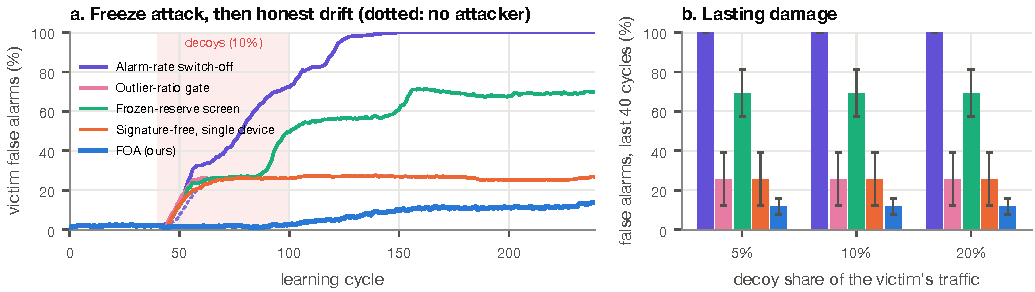
\includegraphics[width=\textwidth]{figures/fig_freeze.pdf}
\caption{Freeze attack. (a) False alarms on the targeted device; decoys from cycle 40 to 100 (10\% share),
honest drift from 40 to 160. Dotted: same rule, no attacker. (b) False alarms over the last 40 cycles
by decoy share.}
\label{fig:freeze}
\end{figure*}

\subsection{Attacks on the gossip}
\textbf{Byzantine peers.} With strong drift, FOA is not compromised with one or two of the victim's
seven peers fully controlled by the attacker (\ByzO, \ByzT), but it is with three (\ByzH), although three
of seven is below the geometric median's breakdown point. This is Theorem~\ref{thm:byz}'s caveat in
practice: during drift the victim agrees with the consensus, so a consistent bias of order $C_\alpha r$
per cycle is applied, and our default common budget is generous enough to let it accumulate. Without
drift the victim's own traffic does not back the biased consensus and no number of Byzantine peers
compromised it. A tighter common budget would trade shared-drift liveness for this case.
\textbf{Keyless attackers.} Twelve forged frames per cycle plus replays of the previous cycle's frames
had no effect (\SybilFOA\ compromised; every forged and replayed frame was rejected). With
authentication switched off, the same attacker compromised the victim in \SybilNoHMAC\ of runs.
\textbf{Lossy radio.} Losing up to 70\% of frames changed little (fleet false alarms \LossNoneFPR\
with no loss, \LossHalfFPR\ at 50\%); at 90\% most cycles have fewer than two peers, FOA falls back to
its residual budget and false alarms rise.

\begin{figure*}[t]
\centering
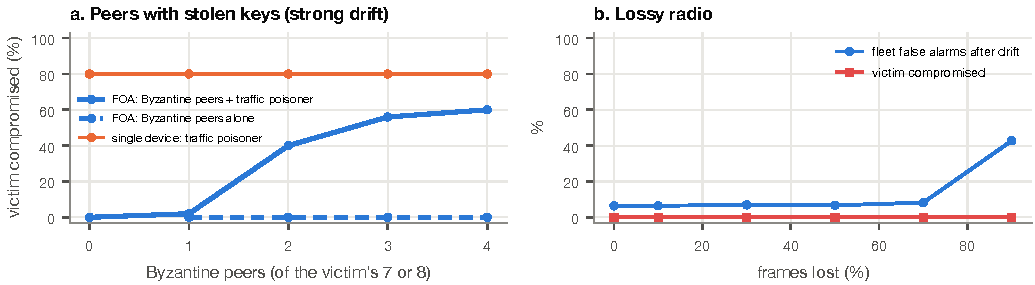
\includegraphics[width=0.8\textwidth]{figures/fig_gossip.pdf}
\caption{Attacks on the gossip. (a) Byzantine peers with valid keys. (b) Frame loss.}
\label{fig:gossip}
\end{figure*}

\subsection{One knob: the residual rate}\label{sec:frontier}
Table~\ref{tab:sweep} sweeps $B$. With $B\le$\SweepSafeMaxB\ alarm radii per cycle no victim was
compromised; larger $B$ admits the attacker faster (\SweepCompHigh\ compromised at $B=0.04$). In
exchange, a device's own drift is followed faster: false alarms after device-only drift fall from
\SweepIdioLow\ at the smallest $B$ to \SweepIdioHigh\ at $B=0.02$. No setting is free, as
Proposition~\ref{prop:frontier} says; the bound of Corollary~\ref{cor:ttc} held in every run of the
sweep (\SweepViol\ violations). Figure~\ref{fig:theory} repeats the sweep on a synthetic fleet with known
geometry and checks the Byzantine lemma numerically.

\begin{figure*}[t]
\centering
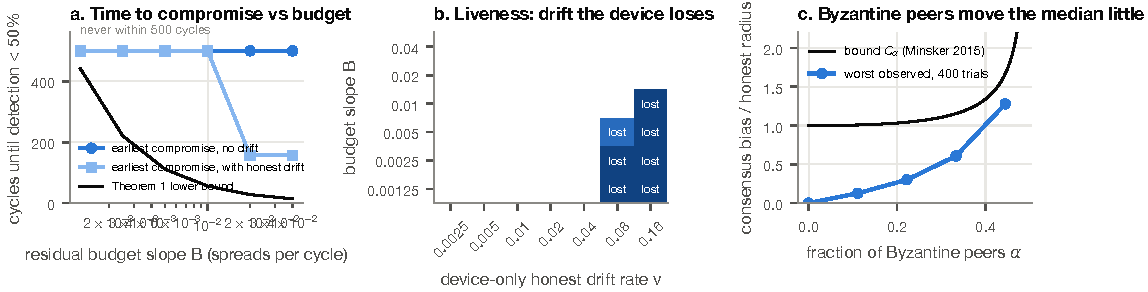
\includegraphics[width=\textwidth]{figures/fig_theory.pdf}
\caption{Theory checks on a synthetic fleet with known geometry. (a) Earliest compromise against the
budget slope, with the closed-form lower bound of Corollary~\ref{cor:ttc}. (b) Device-only drift rates
that a device loses, for each budget slope. (c) Worst observed consensus bias with $f$ Byzantine peers
against Lemma~\ref{lem:gm}.}
\label{fig:theory}
\end{figure*}

\subsection{Ablations and adaptive attackers}\label{sec:ablation}
Table~\ref{tab:ablation} removes one piece at a time. Discarding the residual instead of rationing it
(the CIoTA choice applied to diverse peers) leaves devices unable to follow anything their peers do not
share: fleet false alarms rise to \AblDiscardFPR. Removing the peers (budget only) gives
\AblNoPeersFPR. Removing the residual budget gives back the attack (\AblFullComp\ compromised). Measuring
agreement with a mean instead of a median roughly doubles false alarms (\AblMeanLamFPR\ against
\AblFOAFPR), because an attacker can then cancel the victim's agreement and stall it. A wider spread
budget or a joint centre-and-spread budget lets attackers through: inflating the spread is the cheapest
way to make an attack fit. When a device has its own large drift on top of the shared one, almost every
variant loses that device (false alarms of 74 to 100\%); only the variants with more room (no residual
budget, or one joint budget) partly keep up, and both are poisoned. Removing the residual budget is also
the only change that ever violated the bound of Corollary~\ref{cor:ttc} (4 runs), as it should. Among
adaptive attackers (strong drift, share 0.3, three victims), pulsing compromised no one under either
rule; FOA cut the core-hiding attacker from 33\% to 10\%; and multi-direction, consensus-aligned and
mimicry attackers each compromised one of the three victims (33\%) under both FOA and single-device
adaptation, so FOA did not help against them on that victim.

\subsection{A four-node fleet}
The testbed has four ESP32 nodes. Simulating a fleet of four vendors (Danmini, Ecobee, Provision PT-838,
SimpleHome XCS7-1003) with strong drift and a boundary attacker at share 0.3: FOA \FourCompFOA\
compromised with \FourFPRFOA\ fleet false alarms; single-device adaptation \FourCompAuto\ and
\FourFPRAuto; alarm-rate switch-off \FourCompKL\ and \FourFPRKL; frozen reserve \FourCompFrozen\ and
\FourFPRFrozen. Three peers are enough for the consensus to work. Joining devices were never
compromised in our join experiment (\JoinComp), with or without the warm start.

\subsection{Real drift: 40 weeks of CESNET traffic}\label{sec:cesnet}
The injected drift above is a stress test. To check FOA on drift nobody designed, we use
CESNET-TimeSeries24~\cite{cesnet}: traffic statistics of IP addresses in a national research network
from October 2023 to July 2024, which span a semester, holidays and the institutions' own changes. The
fleet is the twelve most active addresses of one institution (they share its network); a learning cycle
is one day of 10-minute aggregates (twelve statistics: flows, packets, bytes, destinations, ports,
protocol and direction ratios, duration, TTL), the first 28 days calibrate, and 252 days stream. Nothing
about the drift is injected. The attack is modelled, because the dataset has no attack labels: the IP's
own traffic turned into a scanner (twenty times the flows, thirty times the destinations, short flows),
with a boundary poisoner from day 30. Eleven of the twelve addresses meet the victim rule.

The real drift is milder than our stress test: the static detector stays at \CesStaticFPR\ false
alarms, except one address whose behaviour changes for good in the second half and which every rule
loses. Every adaptive rule pays something for adapting to daily variation (single device \CesAutoFPR,
alarm-rate switch-off \CesKLFPR); FOA pays least among the protected rules (\CesFOAFPR). Under attack,
naive learning was compromised in \CesNaiveComp\ of runs, single-device adaptation and the alarm-rate
switch-off in \CesAutoComp\ and \CesKLComp, the frozen reserve in \CesFrozenComp, and FOA in
\CesFOAComp\ (Figure~\ref{fig:cesnet}).

\begin{figure*}[t]
\centering
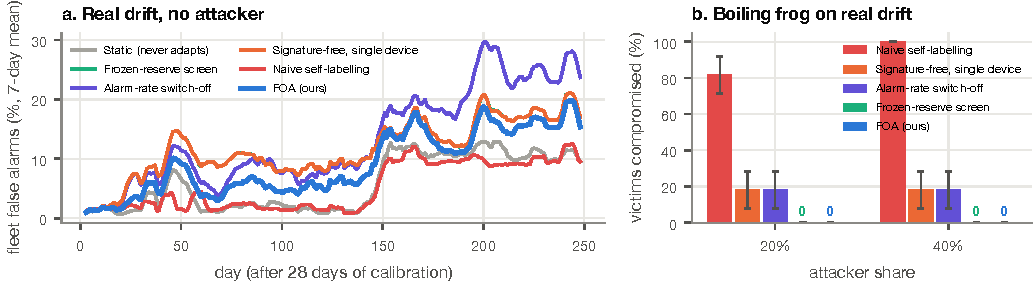
\includegraphics[width=\textwidth]{figures/fig_cesnet.pdf}
\caption{CESNET-TimeSeries24, twelve addresses of one institution, one learning cycle per day.
(a) Fleet false alarms under real drift, no attacker (the frozen reserve never filters here and coincides with single-device adaptation). (b) Victims compromised by a boundary poisoner
(11 victims, 5 held-out seeds).}
\label{fig:cesnet}
\end{figure*}



\subsection{Cost on an ESP32}\label{sec:cost}

FOA's on-device part is about 500 lines of portable C99 with no heap: the detector, the signature-free
proposal with the median agreement projection, ten Weiszfeld iterations, the FOA step, the 92-byte frame
and HMAC-SHA256. Table~\ref{tab:cost} summarises what we could verify before the boards arrived.

\textbf{Equivalence.} On 480 recorded cycles from three synthetic fleets (one with 85\% frame loss, so
130 cycles had fewer than two peers), the C proposal matches the Python reference to a worst relative
error of $5.4\times10^{-4}$ (float32 against float64) and the C FOA step to $6\times10^{-5}$, with zero
mismatches. Frames packed in C are byte-identical to Python's; all 23{,}040 single-bit flips, wrong keys
and stale cycle numbers are rejected; HMAC-SHA256 passes RFC 4231 test case 2.

\textbf{Footprint.} Compiled for the ESP32 (Arduino-ESP32 core 3.3.12) the node firmware uses
915{,}504 bytes of flash and 69{,}216 bytes of static RAM; the same Wi-Fi, UDP and ESP-NOW code without
FOA uses 893{,}284 and 48{,}928. FOA therefore costs about 22\,KB of flash and 20\,KB of static RAM, of
which 13\,KB is the batch of 200 sixteen-dimensional samples; calibration borrows about 80\,KB of heap once and
frees it. The detector and FOA state are 452 bytes.

\textbf{Time and energy (estimates).} On the laptop one proposal over 200 points takes 5\,$\mu$s, one FOA
step with 8 peers 0.7\,$\mu$s and one frame signature 1.2\,$\mu$s. The step is about $3{\times}10^4$
floating-point operations plus a few hundred square roots; at 240\,MHz and a conservative ten cycles per
operation this is about 2\,ms per learning cycle, against a cycle length of 10\,s. One 92-byte ESP-NOW
broadcast per cycle is about 1\,ms of airtime. These are estimates; the firmware logs the measured time
of every stage and the INA219 monitor gives energy per cycle on the testbed.

\begin{table}[t]
\centering
\caption{FOA on the ESP32: verified before hardware, and estimated}
\label{tab:cost}
\small
\begin{tabular}{@{}lr@{}}
\toprule
C vs Python, 480 cycles & 0 mismatches \\
Tampered frames accepted & 0 of 23{,}104 \\
Added flash / static RAM & 22\,KB / 20\,KB \\
State per device & 452 B \\
Gossip per device per cycle & one 92 B frame \\
Compute per cycle (est.) & $\approx$2\,ms at 240\,MHz \\
\bottomrule
\end{tabular}
\end{table}

